\begin{problem}
  Sketch the Lagrange polynomials of degree 3 in a single plot.
\end{problem}

% --------------------------------------------------------------------%
\begin{solution}
  \begin{figure}[!ht]
    \centering
    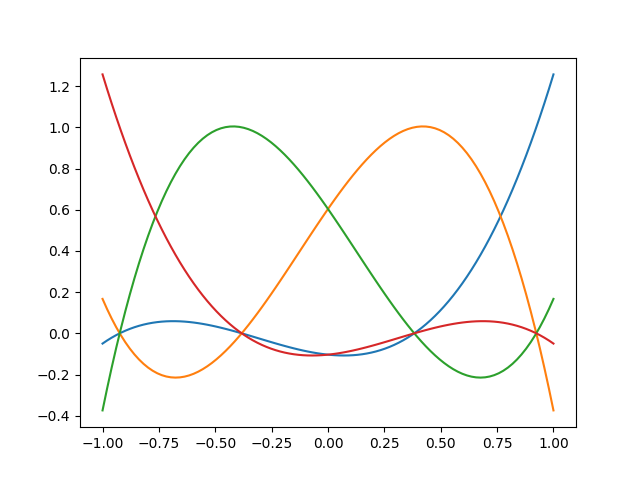
\includegraphics[scale = 0.5]{./code/task_3.png}
    \caption{Lagrange polynomials generated by four Chebyshev points on
      the intervall $[-1, 1]$.}
    \label{fig:3}
  \end{figure}
  Figur~\ref{fig:3} shows the four lagrange polynomials generated
  by four Chebyshev points. It is easy to identify both the polynomials
  as well as the points used. By construction the polynomials have
  property of being 1 at on of the points and 0 at all other.
\end{solution}

%%% Local Variables:
%%% TeX-master: "report.tex"
%%% End:
